\section{Expected Results}

\begin{frame}{Expected Results}

    To summarize, the expected results of this research are:

    \begin{itemize}
        \item<2-> Phase 1: \textbf<2>{Numerical model of the Ammonia dynamics for non-reactive condition}.
        \item<3-> Phase 2: Set of experimental data and \textbf<3>{numerical model of the Ammonia dynamics for reactive condition}.
        \item<4-> Phase 3: \textbf<4>{Fuel injector design for pure Ammonia combustion}.
    \end{itemize}

    \begin{columns}[t, onlytextwidth]

        \begin{column}{0.28\textwidth}

            \onslide<2->{
                \begin{figure}
                    \centering
                    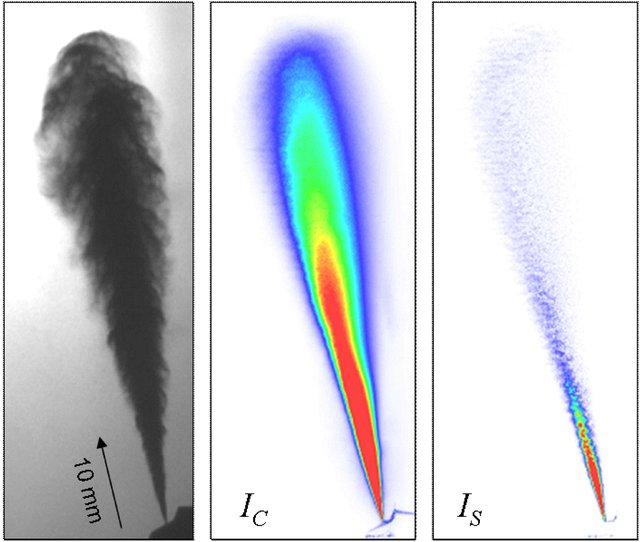
\includegraphics[height=2.6cm]{img/result-phase-1.jpg}
                    \caption{NM\footnotemark[1] (non-reactive condition).}
                \end{figure}
            }

        \end{column}

        \hfill

        \begin{column}{0.28\textwidth}

            \onslide<3->{
                \begin{figure}
                    \centering
                    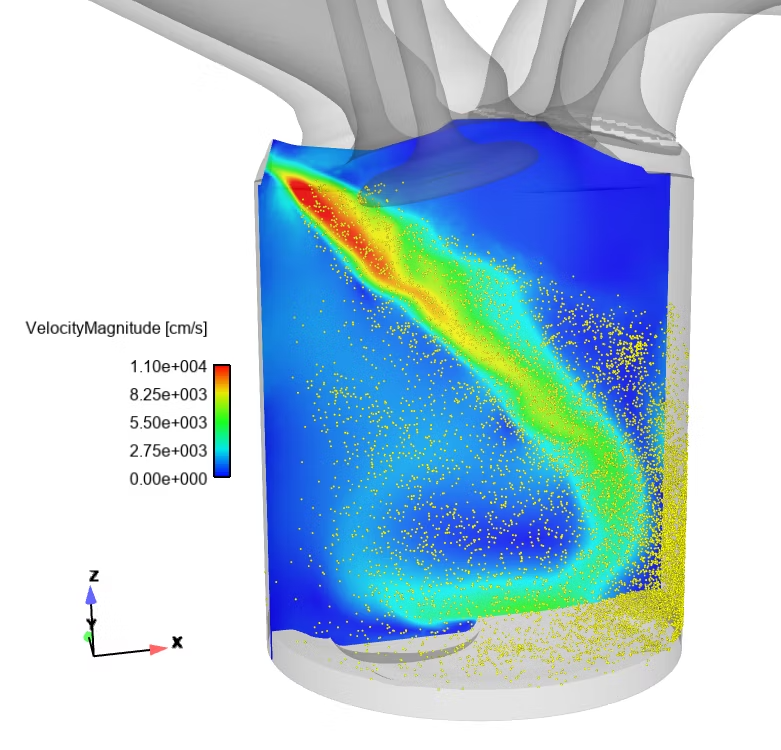
\includegraphics[height=2.6cm]{img/result-phase-2.png}
                    \caption{NM\footnotemark[1] (reactive condition).}
                \end{figure}
            }

        \end{column}

        \hfill

        \begin{column}{0.36\textwidth}

            \onslide<4->{
                \begin{figure}
                    \centering
                    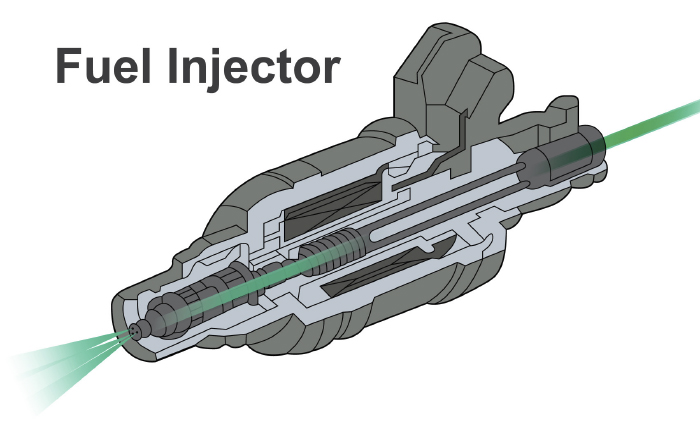
\includegraphics[height=2.6cm]{img/Fuel-injector.jpg}
                    \caption{Fuel injector design.}
                \end{figure}
            }

        \end{column}

    \end{columns}

    \onslide<2->{\footnotetext[1]{NM: Numerical Model.}}

\end{frame}

